%% FEUP THESIS STYLE for LaTeX2e
%% how to use feupteses (portuguese version)
%%
%% FEUP, JCL & JCF, 31 Jul 2012
%%
%% PLEASE send improvements to jlopes at fe.up.pt and to jcf at fe.up.pt
%%

%%========================================
%% Commands: pdflatex pdis
%%           bibtex pdis
%%           makeindex pdis (only if creating an index) 
%%           pdflatex pdis
%% Alternative:
%%          latexmk -pdf pdis.tex
%%========================================

\documentclass[11pt,a4paper,twoside,openright]{report}

%% For iso-8859-1 (latin1), comment next line and uncomment the second line
\usepackage[utf8]{inputenc}
%\usepackage[latin1]{inputenc}

%% Portuguese version

%% MIEIC options
\usepackage[portugues,mieic]{feupteses}
%\usepackage[portugues,mieic,juri]{feupteses}
%\usepackage[portugues,mieic,final]{feupteses}
%\usepackage[portugues,mieic,final,onpaper]{feupteses}

%% Options: 
%% - portugues: titles, etc in portuguese
%% - onpaper: links are not shown (for paper versions)
%% - backrefs: include back references from bibliography to citation place

%% Uncomment the next lines if side by side graphics used
%\usepackage[lofdepth,lotdepth]{subfig}
%\usepackage{graphicx}
%\usepackage{float}

%% Include color package
\usepackage{color}
\definecolor{cloudwhite}{cmyk}{0,0,0,0.025}

%% Include source-code listings package
\usepackage{listings}
\lstset{ %
 language=C,                        % choose the language of the code
 basicstyle=\footnotesize\ttfamily,
 keywordstyle=\bfseries,
 numbers=left,                      % where to put the line-numbers
 numberstyle=\scriptsize\texttt,    % the size of the fonts that are used for the line-numbers
 stepnumber=1,                      % the step between two line-numbers. If it's 1 each line will be numbered
 numbersep=8pt,                     % how far the line-numbers are from the code
 frame=tb,
 float=htb,
 aboveskip=8mm,
 belowskip=4mm,
 backgroundcolor=\color{cloudwhite},
 showspaces=false,                  % show spaces adding particular underscores
 showstringspaces=false,            % underline spaces within strings
 showtabs=false,                    % show tabs within strings adding particular underscores
 tabsize=2,	                    % sets default tabsize to 2 spaces
 captionpos=b,                      % sets the caption-position to bottom
 breaklines=true,                   % sets automatic line breaking
 breakatwhitespace=false,           % sets if automatic breaks should only happen at whitespace
 escapeinside={\%*}{*)},            % if you want to add a comment within your code
 morekeywords={*,var,template,new}  % if you want to add more keywords to the set
}

%% Uncomment next line to set the depth of sectional units listed in the toc
%\setcounter{tocdepth}{3}

%% Uncomment to create an index (at the end of the document)
%\makeindex

%% Path to the figures directory
%% TIP: use folder ``figures'' to keep all your figures
\graphicspath{{figures/}}

%%----------------------------------------
%% TIP: if you want to define more macros, use an external file to keep them
%some macro definitions

% format
\newcommand{\class}[1]{{\normalfont\slshape #1\/}}

% entities
\newcommand{\Feup}{Faculdade de Engenharia da Universidade do Porto}

\newcommand{\svg}{\class{SVG}}
\newcommand{\scada}{\class{SCADA}}
\newcommand{\scadadms}{\class{SCADA/DMS}}

% color
\usepackage{color}
\definecolor{cloudwhite}{cmyk}{0,0,0,0.025}
\usepackage[dvipsnames]{xcolor}

% Code
\newcommand{\code}[1]{\path{#1}}

% Math
\usepackage{amsmath}
\newcommand{\pr}{\mbox{Pr}}
\newcommand{\gFunc}[1][d]{\displaystyle\prod_{j \in (d \cap obs_i)} g_j}

% Listings

\usepackage{listings}
\lstset{ %
 language=C,                        % choose the language of the code
 basicstyle=\footnotesize\ttfamily,
 keywordstyle=\bfseries,
 numbers=left,                      % where to put the line-numbers
 numberstyle=\scriptsize\texttt,    % the size of the fonts that are used for the line-numbers
 stepnumber=1,                      % the step between two line-numbers. If it's 1 each line will be numbered
 numbersep=8pt,                     % how far the line-numbers are from the code
 frame=tb,
 float=htb,
 aboveskip=8mm,
 belowskip=4mm,
 backgroundcolor=\color{cloudwhite},
 showspaces=false,                  % show spaces adding particular underscores
 showstringspaces=false,            % underline spaces within strings
 showtabs=false,                    % show tabs within strings adding particular underscores
 tabsize=2,                     % sets default tabsize to 2 spaces
 captionpos=b,                      % sets the caption-position to bottom
 breaklines=true,                   % sets automatic line breaking
 breakatwhitespace=false,           % sets if automatic breaks should only happen at whitespace
 escapeinside={\%*}{*)},            % if you want to add a comment within your code
 morekeywords={*,var,template,new}  % if you want to add more keywords to the set
}

\lstdefinestyle{npmlog}{
  moredelim=**[is][\color{gray}]{?}{?},
  moredelim=**[is][\color{ForestGreen}]{@}{@},
  moredelim=**[is][\color{purple}]{!}{!},
}

\lstdefinelanguage{Javascript}{
  keywords={break, case, catch, continue, debugger, default, delete, do, else, false, finally, for, function, if, in, instanceof, new, null, return, switch, this, throw, true, try, typeof, var, void, while, with},
  morecomment=[l]{//},
  morecomment=[s]{/*}{*/},
  morestring=[b]',
  morestring=[b]",
  ndkeywords={class, export, boolean, throw, implements, import, this},
  keywordstyle=\color{blue}\bfseries,
  ndkeywordstyle=\color{darkgray}\bfseries,
  identifierstyle=\color{black},
  commentstyle=\color{purple}\ttfamily,
  stringstyle=\color{red}\ttfamily,
  sensitive=true
}
%%----------------------------------------

%%========================================
%% Start of document
%%========================================
\begin{document}

%%----------------------------------------
%% Information about the work
%%----------------------------------------
\title{Software Repository Mining for Estimating Software Component Reliability}
\author{André Duarte - ei11044@fe.up.pt}

%% Uncomment next line for date of submission
%\thesisdate{31 de Julho de 2008}

%% Uncomment next line for copyright text if used
%\copyrightnotice{Nome do Autor, 2008}

\supervisor{Orientador}{Rui Maranhão - rma@fe.up.pt}

%% Uncomment next line if necessary
%\supervisor{Co-orientador}{Nome de Outro Orientador}

%% Uncomment committee stuff in the final version
%\committeetext{Aprovado em provas públicas pelo Júri:}
%\committeemember{Presidente}{Nome do presidente do júri}
%\committeemember{Arguente}{Nome do arguente do júri}
%\committeemember{Vogal}{Nome do vogal do júri}
%\signature

%% Specify cover logo (in folder ``figures'')
\logo{uporto-feup.pdf}

%% Uncomment next line for additional text below the author's name (front page)
\additionalfronttext{Preparação da Dissertação}

%%----------------------------------------
%% Preliminary materials
%%----------------------------------------

% remove unnecessary \include{} commands
\begin{Prolog}
  \chapter*{Abstract}
%\addcontentsline{toc}{chapter}{Abstract}

TODO

\vspace*{10mm}\noindent

\textbf{Keyworks}: \emph{Software-fault Localization}, \emph{Software Repository Mining}, \emph{Machine Learning}, \emph{Classification}

\vspace*{5mm}\noindent

\textbf{Classificação}: \emph{Software and its engineering - Software creation and management - Software verification and validation; Computing methodologies - Machine Learning - Machine Learning Approaches}

\chapter*{Resumo}
%\addcontentsline{toc}{chapter}{Resumo}

Dada a crescente necessidade de identificar a localização dos erros no código fonte de \emph{software}, de forma a facilitar o trabalho dos programadores e a acelerar o processo de desenvolvimento, muitos avanços têm sido feitos na sua automação.

Existem três abordagens principais: \emph{Program-spectra based} (PSB), \emph{Model-based diagnosis} (MDB) e \emph{Program slicing}.

\emph{Barinel}, solução que integra tanto o PSB como o MDB, é, até hoje, com base na investigação feita, a que apresenta melhores resultados. Contudo, a ordenação de conjuntos de candidatos (componentes faltosos) não tem em conta a verdadeira qualidade do componente em causa, mas sim o conjunto de valores que maximizam a probabilidade do conjunto (\emph{Maximum Likehood Estimation} - MLE), devido à dificuldade da sua determinação.

Com esta tese pretende-se colmatar esta falha e contribuir para uma melhor ordenação dos conjuntos, classificando, com recurso a técnicas de Machine Learning como \emph{Naive Bayes}, \emph{Support Vector Machines} (SVM) ou \emph{Random Forests}, a qualidade e fiabilidade de cada componente, através das informações disponíveis no sistema de controlo de versões (\emph{Software Repository Mining}), neste caso \emph{Git}, como por exemplo: número de vezes que foi modificado, número de contribuidores, data de última alteração, nome de últimos contribuidores e tamanho das alterações.

A investigação já feita, revelou a existência de algumas soluções de análise preditiva de \emph{software}, como \emph{BugCache}, \emph{FixCache} e \emph{Change Classification}, capazes de identificar componentes com grande probabilidade de falhar e de classificar as revisões (\emph{commits}) como faltosas ou não, mas nenhuma soluciona o problema.

Este trabalho visa também a integração com o \emph{Crowbar} e a contribuição para a sua possível comercialização.

\vspace*{10mm}\noindent

\textbf{Palavras-chave}: \emph{Software-fault Localization}, \emph{Software Repository Mining}, \emph{Machine Learning}, \emph{Classification}

\vspace*{5mm}\noindent

\textbf{Classificação}: \emph{Software and its engineering - Software creation and management - Software verification and validation; Computing methodologies - Machine Learning - Machine Learning Approaches} % the abstract
  % \chapter*{Agradecimentos}
%\addcontentsline{toc}{chapter}{Agradecimentos}

Aliquam id dui. Nulla facilisi. Nullam ligula nunc, viverra a, iaculis
at, faucibus quis, sapien. Cum sociis natoque penatibus et magnis dis
parturient montes, nascetur ridiculus mus. Curabitur magna ligula,
ornare luctus, aliquam non, aliquet at, tortor. Donec iaculis nulla
sed eros. Sed felis. Nam lobortis libero. Pellentesque
odio. Suspendisse potenti. Morbi imperdiet rhoncus magna. Morbi
vestibulum interdum turpis. Pellentesque varius. Morbi nulla urna,
euismod in, molestie ac, placerat in, orci. 

Ut convallis. Suspendisse luctus pharetra sem. Sed sit amet mi in diam
luctus suscipit. Nulla facilisi. Integer commodo, turpis et semper
auctor, nisl ligula vestibulum erat, sed tempor lacus nibh at
turpis. Quisque vestibulum pulvinar justo. Class aptent taciti
sociosqu ad litora torquent per conubia nostra, per inceptos
himenaeos. Nam sed tellus vel tortor hendrerit pulvinar. Phasellus
eleifend, augue at mattis tincidunt, lorem lorem sodales arcu, id
volutpat risus est id neque. Phasellus egestas ante. Nam porttitor
justo sit amet urna. Suspendisse ligula nunc, mollis ac, elementum
non, venenatis ut, mauris. Mauris augue risus, tempus scelerisque,
rutrum quis, hendrerit at, nunc. Nulla posuere porta orci. Nulla dui. 

Fusce gravida placerat sem. Aenean ipsum diam, pharetra vitae, ornare
et, semper sit amet, nibh. Nam id tellus. Etiam ultrices. Praesent
gravida. Aliquam nec sapien. Morbi sagittis vulputate dolor. Donec
sapien lorem, laoreet egestas, pellentesque euismod, porta at,
sapien. Integer vitae lacus id dui convallis blandit. Mauris non
sem. Integer in velit eget lorem scelerisque vehicula. Etiam tincidunt
turpis ac nunc. Pellentesque a justo. Mauris faucibus quam id
eros. Cras pharetra. Fusce rutrum vulputate lorem. Cras pretium magna
in nisl. Integer ornare dui non pede. 

\vspace{10mm}
\flushleft{O Nome do Autor}
  % the acknowledgments
  % \cleardoublepage
\thispagestyle{plain}

\vspace*{8cm}

\begin{flushright}
   \textsl{``You should be glad that bridge fell down. \\
           I was planning to build thirteen more to that same design''} \\
\vspace*{1.5cm}
           Isambard Kingdom Brunel
\end{flushright}
    % initial quotation if desired
  \cleardoublepage
  \pdfbookmark[0]{Conteúdo}{contents}
  \tableofcontents
  \cleardoublepage
  \pdfbookmark[0]{Lista de Figuras}{figures}
  \listoffigures
  \cleardoublepage
  \pdfbookmark[0]{Lista de Tabelas}{tables}
  \listoftables
  \chapter*{Abreviaturas e Símbolos}
%\addcontentsline{toc}{chapter}{Abbreviations}
\chaptermark{ABREVIATURAS E SÍMBOLOS}

\begin{flushleft}
\begin{tabular}{l p{0.8\linewidth}}
MSR 	 & Mining Software Repositories\\

\end{tabular}
\end{flushleft}

  % the list of abbreviations used
\end{Prolog}

%%----------------------------------------
%% Body
%%----------------------------------------

\StartBody

%% TIP: use a separate file for each chapter
\chapter{Introdução} \label{chap:intro}

\section*{}


\section{Contexto/Enquadramento} \label{sec:context}

Com o elevado crescimento da indústria de desenvolvimento de software,
torna-se cada vez mais importante a existência de ferramentas que auxiliem
os programadores a desenvolvê-lo mais eficientemente.

Estima-se que a economia dos Estados Unidos perca entre 60 mil milhões de dólares por ano em custos associados ao desenvolvimento e distribuição de correções para defeitos de \emph{software} e na sua reinstalação \cite{Zhivich2009}. Pelo que, podemos afirmar que as ferramentas de localização das falhas de \emph{software} (\emph{Software Fault Localization}), ajudando a reduzir o tempo investido nesta tarefa, poderão ter um impacto significativo na economia. % TODO: Citation - The Real Cost of Software Errors
Nesta área os avanços são consideráveis. \emph{Ochiai}, \emph{Tarantula}, \emph{Bayes-A} e \emph{Barinel} são apenas algumas das soluções existentes, sendo o algoritmo \emph{Barinel} aquele que apresenta melhores resultados. \cite{Abreu2009}
Apesar dos bons resultados apresentados pelo \emph{Barinel}, este poderá apresentar resultados ainda mais rigorosos se tivermos informações relativas ao projeto, como a probabilidade média de erro ou a probabilidade de dado componente, que o constitui, ter defeitos.

Ferramentas de controlo de versões, como o \emph{Git}, uma vez que mantêm todo o histórico do projeto e informações relacionadas com as diversas alterações (p.e. conteúdo, data e autores), em conjunto com técnicas de \emph{Machine Learning}, poderão ser a chave para a melhoria deste algoritmo.

\section{Motivação e Objetivos} \label{sec:goals}

Tendo em conta as possibilidades que a extração de dados de repositórios de controlo de versões e o \emph{Machine Learning} nos dão, pretende-se com esta dissertação:

\begin{itemize}
\item Optimizar a ordenação de resultados candidatos do algoritmo Barinel.
\item Ter a capacidade de prever a probabilidade de erro de cada um dos componentes de um dado projecto de \emph{software} que use o \emph{Git} para controlo total de versões, com uma precisão útil.
\end{itemize}

% TODO: Deve ser mesmo "da Dissertação" ??
\section{Estrutura da Dissertação} \label{sec:struct}

Para além da introdução, esta dissertação contém mais 3 capítulos.
No capítulo~\ref{chap:sota}, é descrito o estado da arte e são
apresentados trabalhos relacionados. 

% TODO!!
\textbf{\textcolor{red}{Completar, quando terminar} }
 
\chapter{Revisão Bibliográfica} \label{chap:sota}

\section*{}

Neste capítulo é descrito o estado da arte e são
apresentados trabalhos relacionados para mostrar o que existe no
mesmo domínio e quais os problemas em aberto.
Deve deixar claro que existe uma oportunidade de desenvolvimento que
cobre alguma falha concreta .

O capítulo deve também efetuar uma revisão tecnológica às principais
ferramentas utilizáveis no âmbito do projeto, justificando futuras
escolhas.

\section{Introdução}

Neste capítulo é ilustrada a utilização de macros \LaTeX\ para definir
entradas no índice remissivo e são feitas diversas referências
bibliográficas, usando-se texto de um artigo apresentado na Conferência 
XATA2006~\cite{kn:MVL06-xata}.

Nos últimos tempos têm surgido diversas soluções, apresentadas por
empresas do sector Automação de Sistemas para a disponibilização de
sistemas \scadadms{} na \textit{Web}.

Aliquam sollicitudin facilisis sapien. Mauris tincidunt tristique
diam. Mauris sollicitudin pede at tellus varius volutpat. Integer vel
leo. Nunc massa diam, egestas eu, venenatis at, porttitor ac,
sapien. Sed magna elit, vulputate in, lacinia sed, lobortis ac,
urna. Proin cursus massa id risus. Vestibulum libero. Curabitur
venenatis augue. Mauris eu libero eget lectus tempus tempor. In
tincidunt, justo in varius adipiscing, ipsum enim gravida massa, eget
ornare ante lacus id est. Praesent vitae est ut elit convallis
convallis. Aenean tincidunt, purus id consectetur volutpat, sem leo
pulvinar libero, nec semper sem purus ultricies nibh \cite{kn:Fra94-thesis}. 

Fusce risus mi, tristique eu, consectetuer id, auctor sed, elit. Donec
laoreet. Duis consectetuer interdum libero. Etiam eu orci. In eu
arcu. Fusce luctus diam eget lectus. Duis interdum lacus sed
ligula. Proin vestibulum felis eget lacus. Vivamus vestibulum, tellus
ut congue viverra, mauris lacus tempor turpis, eu congue nisi magna at
dolor. Ut molestie vehicula libero. Praesent in neque sed risus tempus
ornare. Donec hendrerit, erat eu semper aliquam, pede nulla dapibus
risus, ut pretium orci pede et neque.
Etiam eget tortor a metus convallis viverra. Quisque eget nisi sed
orci facilisis interdum. Aliquam non felis. 

\section{Secção Exemplo}\label{sec:dialecto}

\emph{Scalable Vector Graphics}\index{SVG}\index{XML!SVG} é uma
linguagem em formato XML que descreve gráficos de duas dimensões. 
Este formato padronizado pela W3C (\emph{World Wide Web Consortium})
é livre de patentes ou direitos de autor e está totalmente
documentado, à semelhança de outros W3C
standards~\cite{kn:svgdoc}.

Sendo uma linguagem XML, o \svg{} herda uma série de vantagens: a
possibilidade de transformar \svg{} usando técnicas como
XSLT\index{XML!XSLT}, de embeber \svg{} em qualquer documento
XML\index{XML} usando \textit{namespaces} ou até de  
estilizar \svg{} recorrendo a CSS\index{CSS} (\emph{Cascade Style Sheets}). 
De uma forma geral, pode dizer-se que \svg{}s interagem bem com as
atuais tecnologias ligadas ao XML e à Web, tal como referido
em~\cite{kn:svgibm,kn:svgw3c}.

Lorem ipsum dolor sit amet, consectetuer adipiscing elit. Donec a
eros. Phasellus non nulla non massa venenatis convallis. In
porta. Mauris quis magna. Proin mauris eros, aliquet id, eleifend
vitae, semper quis, erat. Aliquam id lectus non odio dignissim
blandit. Vestibulum porttitor arcu ut ligula. Nunc quis
erat. Curabitur ipsum tortor, ornare vitae, dapibus pretium, hendrerit
sed, urna. Vestibulum ante ipsum primis in faucibus orci luctus et
ultrices posuere cubilia Curae; Phasellus bibendum, nulla eget varius
aliquam, tortor nulla sollicitudin quam, vel vestibulum nisl magna at
sem. Aliquam velit sapien, ultrices viverra, tempus quis, ultrices at,
dui. Aliquam sit amet justo. 

Quisque tristique, metus eu iaculis
sagittis, urna leo bibendum diam, a ultricies sem diam a augue. Mauris
consectetuer, libero vel euismod tincidunt, nisi metus viverra ante,
quis pretium sapien odio nec risus. Nunc semper auctor
nulla\footnote{Exemplo de nota de rodapé.}. 

\subsection{Subsecção Exemplo} \label{batik} 

Batik é um conjunto de bibliotecas baseadas em \textit{Java} que
permitem o uso de imagens \svg{} (visualização, geração ou
manipulação) em aplicações ou \textit{applets}~\cite{kn:batik}.  
O projeto Batik\index{Batik} destina-se a fornecer ao programador
alguns módulos que permitem desenvolver soluções especificas usando
\svg~\cite{kn:svgdoc}. 

Lorem ipsum dolor sit amet, consectetuer adipiscing elit. Nunc eu
nulla. Pellentesque vitae nibh ultrices quam iaculis
convallis. Aliquam purus eros, varius eget, volutpat sodales,
imperdiet nec, lacus. Curabitur in elit sed sem rutrum posuere. Class
aptent taciti sociosqu ad litora torquent per conubia nostra, per
inceptos himenaeos. Duis sem. Praesent ultricies odio vel
sapien. Integer faucibus malesuada libero. Cras semper, dolor id
ullamcorper varius, magna risus volutpat felis, id pellentesque nulla
ante at erat. Integer sodales. 

Quisque sit amet odio. In at risus sit amet turpis interdum
posuere. Maecenas iaculis vehicula sem. Ut leo arcu, malesuada vel,
imperdiet id, dignissim a, purus. Duis eleifend, lectus non venenatis
dignissim, risus libero imperdiet mi, nec gravida massa libero sed
mauris. Nullam lobortis libero non sapien. Integer convallis iaculis
erat. Morbi dictum. Ut ultrices pellentesque velit. Cras ac
ante. Etiam in neque tincidunt lacus gravida vehicula. Proin et nisi. 

\subsection{Subsecção Exemplo}

Loren ipsum dolor sit amet, consectetuer adipiscing elit. 
Praesent sit amet sem. Maecenas eleifend facilisis leo. Vestibulum et
mi. Aliquam posuere, ante non tristique consectetuer, dui elit
scelerisque augue, eu vehicula nibh nisi ac est. Suspendisse elementum
sodales felis. Nullam laoreet fermentum urna. 

Loren ipsum dolor sit amet, consectetuer adipiscing elit. 
Praesent sit amet sem. Maecenas eleifend facilisis leo. Vestibulum et
mi. Aliquam posuere, ante non tristique consectetuer, dui elit
scelerisque augue, eu vehicula nibh nisi ac est. Suspendisse elementum
sodales felis. Nullam laoreet fermentum urna. 

Duis eget diam. In est justo, tristique in, lacinia vel, feugiat eget,
quam. Pellentesque habitant morbi tristique senectus et netus et
malesuada fames ac turpis egestas. Fusce feugiat, elit ac placerat
fermentum, augue nisl ultricies eros, id fringilla enim sapien eu
felis. Vestibulum ante ipsum primis in faucibus orci luctus et
ultrices posuere cubilia Curae; Sed dolor mi, porttitor quis,
condimentum sed, luctus in. 

\section{Resumo ou Conclusões}

No final do capítulo deverá ser apresentado um resumo com as 
principais conclusões que se podem tirar. 

Vivamus non nunc nec risus tempor varius. Quisque bibendum mi at
dolor. Aliquam consectetuer condimentum risus. Aliquam luctus pulvinar
sem. Duis aliquam, urna et vulputate tristique, dui elit aliquet nibh,
vel dignissim magna turpis id sapien. Duis commodo sem id
quam. Phasellus dolor. Class aptent taciti sociosqu ad litora torquent
per conubia nostra, per inceptos himenaeos. 

\chapter{Visualização de Sinópticos SVG}\label{chap:chap3}

\section*{}

Este capítulo deve começar por fazer uma apresentação detalhada do
problema a resolver\footnote{Na introdução a apresentação do
  problema foi breve.} podendo mesmo, caso se justifique,
constituir-se um capítulo com essa finalidade.

Deve depois dedicar-se à apresentação da solução sem detalhes de
implementação. 
Dependendo do trabalho, pode ser uma descrição mais teórica, mais
``arquitetural'', etc.

\section{Secção Exemplo}

Neste capítulo apresentam-se exemplos de formatação de figuras e
tabelas, equações e referências cruzadas.

Apresenta-se de seguida um exemplo de equação, completamente fora do contexto:
\begin{eqnarray}
CIF_1: \hspace*{5mm}F_0^j(a) &=& \frac{1}{2\pi \iota} \oint_{\gamma} \frac{F_0^j(z)}{z - a} dz\\
CIF_2: \hspace*{5mm}F_1^j(a) &=& \frac{1}{2\pi \iota} \oint_{\gamma} \frac{F_0^j(x)}{x - a} dx \label{eq:cif}
\end{eqnarray}

Na Equação~\ref{eq:cif} lorem ipsum dolor sit amet, consectetuer
adipiscing elit. Suspendisse tincidunt viverra elit. Donec tempus
vulputate mauris. Donec arcu. Vestibulum condimentum porta
justo. Curabitur ornare tincidunt lacus. Curabitur ac massa vel ante
tincidunt placerat. Cras vehicula semper elit. Curabitur gravida, est
a elementum suscipit, est eros ullamcorper quam, sed cursus velit
velit tempor neque. Duis tempor condimentum ante.

Phasellus imperdiet, orci vel pretium sollicitudin, magna nunc
ullamcorper augue, non venenatis dui nunc quis massa. Pellentesque
dolor elit, dapibus venenatis, viverra ultricies, accumsan cursus,
orci. Aliquam erat volutpat. Mauris ornare tristique leo. Maecenas
eros. Curabitur velit nunc, tincidunt vitae, dictum posuere, pulvinar
nec, diam. In suscipit mauris a nunc. Pellentesque gravida. Morbi quam
lacus, pretium eget, tincidunt vulputate, interdum sed,
turpis. Curabitur quis est. Sed lectus lorem, congue vel, dignissim
laoreet, blandit a, nisi. Aenean nunc ligula, tincidunt eu, hendrerit
vel, suscipit non, erat. Aliquam gravida. Integer non pede. In laoreet
augue id leo. Mauris placerat. 

A arquitetura do visualizador assenta sobre os seguintes conceitos
base~\cite{kn:ZPMD97}: 

\begin{itemize}
\item \textbf{Componentes} --- Suspendisse auctor mattis augue \emph{push};
\item \textbf{Praesent} --- Sit amet sem maecenas eleifend facilisis leo;
\item \textbf{Pellentesque} --- Habitant morbi tristique senectus et netus.
\end{itemize}

\subsection{Exemplo de Figura}

É apresentado na Figura~\ref{fig:arch} %da página~\pageref{fig:arch}
um exemplo de figura flutuante.

\begin{figure}[t]
  \begin{center}
    \leavevmode
    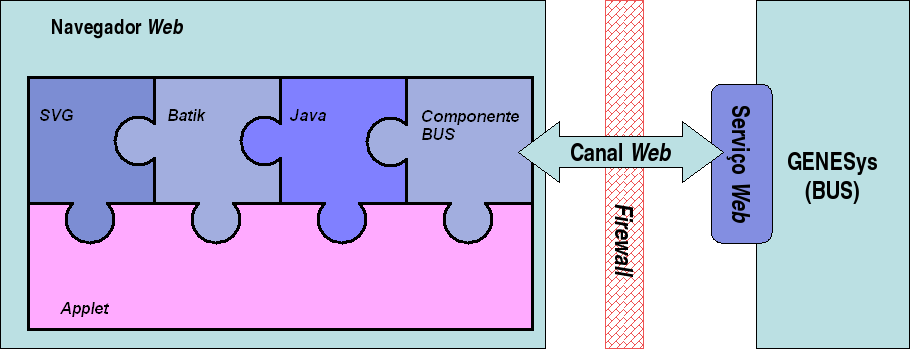
\includegraphics[width=0.86\textwidth]{puzzle}
    \caption{Arquitectura da Solução Proposta}
    \label{fig:arch}
  \end{center}
\end{figure}

Loren ipsum dolor sit amet, consectetuer adipiscing elit. 
Praesent sit amet sem. Maecenas eleifend facilisis leo. Vestibulum et
mi. Aliquam posuere, ante non tristique consectetuer, dui elit
scelerisque augue, eu vehicula nibh nisi ac est. Suspendisse elementum
sodales felis. Nullam laoreet fermentum urna. 

Duis eget diam. In est justo, tristique in, lacinia vel, feugiat eget,
quam. Pellentesque habitant morbi tristique senectus et netus et
malesuada fames ac turpis egestas. Fusce feugiat, elit ac placerat
fermentum, augue nisl ultricies eros, id fringilla enim sapien eu
felis. Vestibulum ante ipsum primis in faucibus orci luctus et
ultrices posuere cubilia Curae; Sed dolor mi, porttitor quis,
condimentum sed luctus. 

\subsection{Exemplo de Tabela}

É apresentado na Tabela~\ref{tab:exemplo1} um exemplo de tabela
flutuante e na Tabela~\ref{tab:exemplo2} um exemplo de tabela
flutuante, um pouco mais complicada.

\begin{table}[t]
  \centering
  \caption{Uma Tabela Simples}
\begin{tabular}{| l | p{45mm} |}
	\hline
\textbf{Acrónimo} & \textbf{Significado}\\
	\hline
	\hline
        ADT   & \emph{Abstract Data Type}\\\hline
        ANDF  & \emph{Architecture-Neutral Distribution Format}\\\hline
        API   & \emph{Application Programming Interface}\\
	\hline
\end{tabular}
  \label{tab:exemplo1}
\end{table}

Integer quis pede. Fusce nibh. Fusce nec erat vel mi condimentum
convallis. Sed at tortor non mauris pretium aliquet. In in lacus in
dolor molestie dapibus. Suspendisse potenti. Pellentesque sagittis
porta erat. Mauris sodales sapien id augue. Nam eu dolor. Donec sit
amet turpis non orci rhoncus commodo. Etiam condimentum commodo
libero.

Mauris pede. Curabitur faucibus dictum nibh. Proin tincidunt diam
vitae mauris. Sed hendrerit dolor vel ipsum. Nullam dapibus. Vivamus
tellus diam, egestas sit amet, vulputate non, vulputate id, eros. Nunc
sit amet nibh eget nibh imperdiet ornare. Cras vehicula mattis
ipsum. Sed diam arcu, semper at, gravida vitae, fermentum et,
nulla. Aenean massa orci, tristique nec, rutrum id, fringilla eget,
erat. Curabitur nulla ipsum, aliquam sed, rutrum vitae, semper quis,
ante. Fusce at nunc in dolor condimentum tempor. Duis sit amet massa. 

Curabitur convallis nulla quis risus. Nulla mollis porttitor
purus. Fusce ultricies odio at ligula pellentesque suscipit. Nulla
velit libero, blandit a, aliquet quis, hendrerit id, arcu. Phasellus
porttitor porttitor purus. Suspendisse velit tortor, fringilla sit
amet, commodo a, ultrices et, mi. Donec eu metus in erat ornare
adipiscing. Praesent varius mi ac nunc. Vestibulum leo lacus,
elementum in, vestibulum sit amet, hendrerit at, justo. Sed sit amet
neque. Donec libero risus, commodo sit amet, dignissim ut, tincidunt
a, eros. Ut non lacus quis tortor mattis ullamcorper. Vivamus
consequat augue vel erat. Sed tincidunt. Sed leo eros, ornare a,
pulvinar non, mattis quis, nibh. Aliquam faucibus mi ac nisi.

Pellentesque habitant morbi tristique senectus et netus et malesuada
fames ac turpis egestas. Duis aliquet, libero sit amet ornare viverra,
augue erat interdum dolor, vitae tincidunt lorem erat a lacus. Sed
lectus nisi, auctor in, hendrerit a, molestie vel, lectus. Cum sociis
natoque penatibus et magnis dis parturient montes, nascetur ridiculus
mus. Duis lacinia tempor dui. Vivamus rhoncus, tellus a viverra
dignissim, pede dui adipiscing odio, non faucibus metus mi gravida
eros. Nullam a tellus ut velit elementum tempus. Aenean rutrum
convallis tellus. Vestibulum nulla ante, dapibus ut, lobortis ut,
varius sed, nisl. Fusce lobortis. Sed ac lorem. Nulla tincidunt nulla
eget leo. Maecenas ac lectus eu neque ultrices pharetra. Curabitur a
risus nec arcu placerat tempor. Suspendisse magna nisl, viverra a,
adipiscing eget, ornare ultricies, ligula. Maecenas eu ligula vitae
eros convallis dignissim. 

\begin{table}[t]
  \centering
  \caption{Uma Tabela Mais Complicada}
\begin{tabular}{|c|r@{.}lr@{.}lr@{.}l||r|}
	\hline
\multicolumn{8}{|c|}
	{\rule[-3mm]{0mm}{8mm}Iteração $k$ de $f(x_n)$} \\
\textbf{\em k}
	& \multicolumn{2}{c}{$x_1^k$}
	& \multicolumn{2}{c}{$x_2^k$}
	& \multicolumn{2}{c||}{$x_3^k$}
	& comentários \\ \hline \hline
0   & -0&3                 & 0&6                 &  0&7   & - \\
1   &  0&47102965 & 0&04883157 & -0&53345964  & $\delta<\epsilon$ \\
2   &  0&49988691 & 0&00228830 & -0&52246185  & $\delta < \varepsilon$ \\
3   &  0&49999976 & 0&00005380 & -0&523656   &   $N$ \\
4   &  0&5                 & 0&00000307 & -0&52359743  & \\
\vdots	& \multicolumn{2}{c}{\vdots}
	& \multicolumn{2}{c}{$\ddots$}
	& \multicolumn{2}{c||}{\vdots}  & \\
7   &  0&5   & 0&0    & \textbf{-0}&\textbf{52359878}
		 & $\delta<10^{-8}$ \\ \hline
\end{tabular}
  \label{tab:exemplo2}
\end{table}

Loren ipsum dolor sit amet, consectetuer adipiscing elit. 
Praesent sit amet sem. Maecenas eleifend facilisis leo. Vestibulum et
mi. Aliquam posuere, ante non tristique consectetuer, dui elit
scelerisque augue, eu vehicula nibh nisi ac est. Suspendisse elementum
sodales felis. Nullam laoreet fermentum urna. 

Duis eget diam. In est justo, tristique in, lacinia vel, feugiat eget,
quam. Pellentesque habitant morbi tristique senectus et netus et
malesuada fames ac turpis egestas. Fusce feugiat, elit ac placerat
fermentum, augue nisl ultricies eros, id fringilla enim sapien eu
felis. Vestibulum ante ipsum primis in faucibus orci luctus et
ultrices posuere cubilia Curae; Sed dolor mi, porttitor quis,
condimentum sed luctus. 

\section{Secção Exemplo}

Loren ipsum dolor sit amet, consectetuer adipiscing elit. 
Praesent sit amet sem. Maecenas eleifend facilisis leo. Vestibulum et
mi. Aliquam posuere, ante non tristique consectetuer, dui elit
scelerisque augue, eu vehicula nibh nisi ac est. Suspendisse elementum
sodales felis. Nullam laoreet fermentum urna. 

Duis eget diam. In est justo, tristique in, lacinia vel, feugiat eget,
quam. Pellentesque habitant morbi tristique senectus et netus et
malesuada fames ac turpis egestas. Fusce feugiat, elit ac placerat
fermentum, augue nisl ultricies eros, id fringilla enim sapien eu
felis. Vestibulum ante ipsum primis in faucibus orci luctus et
ultrices posuere cubilia Curae; Sed dolor mi, porttitor quis,
condimentum sed luctus. 

\section{Resumo e Conclusões}

Resumir e apresentar as conclusões que se podem tirar no fim deste
capítulo.

\chapter{Validação}\label{chap:chap4}

\section*{}

\chapter{Conclusões} \label{chap:concl}

\section*{}
 

%% Comment next 2 commands if numbered appendices are not used
\appendix
\chapter{Loren Ipsum} \label{ap1:loren}

Depois das conclusões e antes das referências bibliográficas,
apresenta-se neste anexo numerado o texto usado para preencher a
dissertação.

\section{O que é o \emph{Loren Ipsum}?}

\emph{\textbf{Lorem Ipsum}} is simply dummy text of the printing and
typesetting industry. Lorem Ipsum has been the industry's standard
dummy text ever since the 1500s, when an unknown printer took a galley
of type and scrambled it to make a type specimen book. It has survived
not only five centuries, but also the leap into electronic
typesetting, remaining essentially unchanged. It was popularised in
the 1960s with the release of Letraset sheets containing Lorem Ipsum
passages, and more recently with desktop publishing software like
Aldus PageMaker including versions of Lorem Ipsum~\citep{kn:Lip08}. 

\section{De onde Vem o Loren?}

Contrary to popular belief, Lorem Ipsum is not simply random text. It
has roots in a piece of classical Latin literature from 45 BC, making
it over 2000 years old. Richard McClintock, a Latin professor at
Hampden-Sydney College in Virginia, looked up one of the more obscure
Latin words, consectetur, from a Lorem Ipsum passage, and going
through the cites of the word in classical literature, discovered the
undoubtable source. Lorem Ipsum comes from sections 1.10.32 and
1.10.33 of ``de Finibus Bonorum et Malorum'' (The Extremes of Good and
Evil) by Cicero, written in 45 BC. This book is a treatise on the
theory of ethics, very popular during the Renaissance. The first line
of Lorem Ipsum, ``Lorem ipsum dolor sit amet\ldots'', comes from a line in
section 1.10.32.

The standard chunk of Lorem Ipsum used since the 1500s is reproduced
below for those interested. Sections 1.10.32 and 1.10.33 from ``de
Finibus Bonorum et Malorum'' by Cicero are also reproduced in their
exact original form, accompanied by English versions from the 1914
translation by H. Rackham.

\section{Porque se usa o Loren?}

It is a long established fact that a reader will be distracted by the
readable content of a page when looking at its layout. The point of
using Lorem Ipsum is that it has a more-or-less normal distribution of
letters, as opposed to using ``Content here, content here'', making it
look like readable English. Many desktop publishing packages and web
page editors now use Lorem Ipsum as their default model text, and a
search for ``lorem ipsum'' will uncover many web sites still in their
infancy. Various versions have evolved over the years, sometimes by
accident, sometimes on purpose (injected humour and the like). 

\section{Onde se Podem Encontrar Exemplos?}

There are many variations of passages of Lorem Ipsum available, but
the majority have suffered alteration in some form, by injected
humour, or randomised words which don't look even slightly
believable. If you are going to use a passage of Lorem Ipsum, you need
to be sure there isn't anything embarrassing hidden in the middle of
text. All the Lorem Ipsum generators on the Internet tend to repeat
predefined chunks as necessary, making this the first true generator
on the Internet. It uses a dictionary of over 200 Latin words,
combined with a handful of model sentence structures, to generate
Lorem Ipsum which looks reasonable. The generated Lorem Ipsum is
therefore always free from repetition, injected humour, or
non-characteristic words etc. 


%%----------------------------------------
%% Final materials
%%----------------------------------------

%% Bibliography
%% Comment the next command if BibTeX file not used, 
%% Assumes that bibliography is in ``myrefs.bib''
\PrintBib{myrefs}

%% Index
%% Uncomment next command if index is required, 
%% don't forget to run ``makeindex pdis'' command
%\PrintIndex

\end{document}
